\documentclass[twoside]{article}
\setlength{\oddsidemargin}{0.25 in}
\setlength{\evensidemargin}{-0.25 in}
\setlength{\topmargin}{-0.6 in}
\setlength{\textwidth}{6.5 in}
\setlength{\textheight}{8.5 in}
\setlength{\headsep}{0.75 in}
\setlength{\parindent}{0 in}
\setlength{\parskip}{0.1 in}

\usepackage{graphicx}
\usepackage{url}

%
% The following commands sets up the lecnum (lecture number)
% counter and make various numbering schemes work relative
% to the lecture number.
%
\newcounter{lecnum}
\renewcommand{\thepage}{\thelecnum-\arabic{page}}
\renewcommand{\thesection}{\thelecnum.\arabic{section}}
\renewcommand{\theequation}{\thelecnum.\arabic{equation}}
\renewcommand{\thefigure}{\thelecnum.\arabic{figure}}
\renewcommand{\thetable}{\thelecnum.\arabic{table}}
\newcommand{\dnl}{\mbox{}\par}

%
% The following macro is used to generate the header.
%
\newcommand{\lecture}[4]{
  \pagestyle{myheadings}
  \thispagestyle{plain}
  \newpage
  \setcounter{lecnum}{#1}
  \setcounter{page}{1}
  \noindent
  \begin{center}
  \framebox{
     \vbox{\vspace{2mm}
   \hbox to 6.28in { {\bf CMPSCI~377~~~Operating Systems
                       \hfill Fall 2009} }
      \vspace{4mm}
      \hbox to 6.28in { {\Large \hfill Lecture #1  \hfill} }
%       \hbox to 6.28in { {\Large \hfill Lecture #1: #2  \hfill} }
      \vspace{2mm}
      \hbox to 6.28in { {\it Lecturer: #3 \hfill Scribe: #4} }
     \vspace{2mm}}
  }
  \end{center}
  \markboth{Lecture #1: #2}{Lecture #1: #2}
  \vspace*{4mm}
}

%
% Convention for citations is authors' initials followed by the year.
% For example, to cite a paper by Leighton and Maggs you would type
% \cite{LM89}, and to cite a paper by Strassen you would type \cite{S69}.
% (To avoid bibliography problems, for now we redefine the \cite command.)
%
\renewcommand{\cite}[1]{[#1]}

% \input{epsf}

%Use this command for a figure; it puts a figure in wherever you want it.
%usage: \fig{NUMBER}{FIGURE-SIZE}{CAPTION}{FILENAME}
\newcommand{\fig}[4]{
           \vspace{0.2 in}
           \setlength{\epsfxsize}{#2}
           \centerline{\epsfbox{#4}}
           \begin{center}
           Figure \thelecnum.#1:~#3
           \end{center}
   }

% Use these for theorems, lemmas, proofs, etc.
\newtheorem{theorem}{Theorem}[lecnum]
\newtheorem{lemma}[theorem]{Lemma}
\newtheorem{proposition}[theorem]{Proposition}
\newtheorem{claim}[theorem]{Claim}
\newtheorem{corollary}[theorem]{Corollary}
\newtheorem{definition}[theorem]{Definition}
\newenvironment{proof}{{\bf Proof:}}{\hfill\rule{2mm}{2mm}}

% Some useful equation alignment commands, borrowed from TeX
\makeatletter
\def\eqalign#1{\,\vcenter{\openup\jot\m@th
 \ialign{\strut\hfil$\displaystyle{##}$&$\displaystyle{{}##}$\hfil
     \crcr#1\crcr}}\,}
\def\eqalignno#1{\displ@y \tabskip\@centering
 \halign to\displaywidth{\hfil$\displaystyle{##}$\tabskip\z@skip
   &$\displaystyle{{}##}$\hfil\tabskip\@centering
   &\llap{$##$}\tabskip\z@skip\crcr
   #1\crcr}}
\def\leqalignno#1{\displ@y \tabskip\@centering
 \halign to\displaywidth{\hfil$\displaystyle{##}$\tabskip\z@skip
   &$\displaystyle{{}##}$\hfil\tabskip\@centering
   &\kern-\displaywidth\rlap{$##$}\tabskip\displaywidth\crcr
   #1\crcr}}
\makeatother

% **** IF YOU WANT TO DEFINE ADDITIONAL MACROS FOR YOURSELF, PUT THEM HERE:

\usepackage{amsmath}

% Some general latex examples and examples making use of the
% macros follow.

\begin{document}

%FILL IN THE RIGHT INFO.
%\lecture{**LECTURE-NUMBER**}{**DATE**}{**LECTURER**}{**SCRIBE**}
\lecture{6}{Feb 16}{Emery Berger}{Sandeep P, Li Mi}


\section{Amdahl's Law for multi-processors}
 
\begin{figure}[h]
\centering
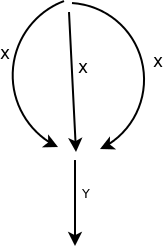
\includegraphics[scale=.70]{Diagram1.png}
\caption{Paths in a program \label{Program}}
\end{figure}
Let x be the time taken by the parallel part of the program . \\
Let y be the time taken by the sequential part of the program . \\
Time taken on a uniprocessor system = 3x+y \\
Time taken on a \infty	processor system = x+y \\
	\frac{T_{1}}{T_{\infty}}=\frac{3x+y}{x+y}

The speedup achieved by parallel processing is bounded by the sequential 
part of the program .
\begin{align}
	T_{p} &= Time\ on\ p\ processors \\
	T_{1} &= Time\ on\ 1\ processors	\\
	T_{\infty} &= Time\ on\ p\ processors \\
	T_{p} &=\frac{T_{1}}{p} + \mathcal{O}(T_{\infty})
\end{align}
As the serial part increases speed up is not achieved due to contention

\section{Pure Private Heap}

If the entire heap is controlled by a single lock . Memory allocation 
becomes sequential as all threads contend for the same lock .An alternative 
to this is every thread having its own private heap . If the objects are 
moved between threads . The private of one thread keeps running out of
memory and the thread which recieves memory from this thread keeps
gaining memory . This results in an unbounded worst case .
\begin{figure}[h]
\centering
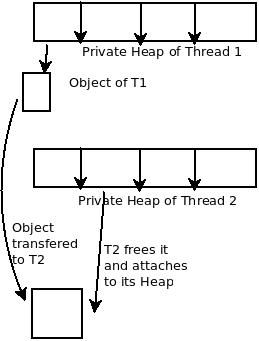
\includegraphics[scale=.50]{Diagram2.jpeg}
\caption{Worst Case Private Heap \label{Worst Case Private Heap}}
\end{figure}

\section{Fragmentation}
\begin{figure}[h]
\centering
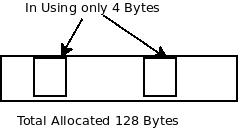
\includegraphics[scale=.50]{Diagram3.jpeg}
\caption{Fragmentation \label{Fragmentation}}
\end{figure}
Allocated memory is 128 bytes while the actual memory 
in use is only 8 bytes , therefore fragmentation is 128/8 .\\
If all objects are of the same size , then it is guaranteed perfect fit.

	\begin{align}
		Fragmentation&=(\frac{A}{U}) \\
		A&=D\ memory\ in\ bytes \\
		U&=memory\ in\ use	\\
	\end{align}
The best memory allocator will suffer a fragmentation of 
	\begin{align}
		&\mathcal{O}(log(\frac{M}{m})) \\
		M&=max\ size\ of\ allocated\ object	\\
		m&=max\ size\ osf\ allocated\ object	\\
	\end{align}
\section{parallel Allocator}
\begin{figure}[h]
\centering
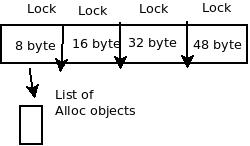
\includegraphics[scale=.50]{Diagram4.jpeg}
\caption{Parallel Allocator \label{Parallel Allocator}}
\end{figure}
Other alternatives to prevent fragmentation. \\
Divide memory into chunks of 8,16,32.. bytes. \\
Each chunk of memory has a lock .

\end{document}
